\section{Kódování a kryptografie}

\subsection{Úvod}

\subsubsection*{Znenie otázky}

Kódování, kryptografie a kryptografické protokoly. Lineární 
kódy (definice, vlastnosti, kódování a dekódování, důležité příklady 
lineárních kódů; cyklické kódy (definice, algebraická charakterizace, 
kódování a dekódování, důležité příklady cyklických kódů); turbo 
kódy a low-density kódy; kryptosystémy s privátním klíčem; DES a AES 
kryptosystémy; kryptosystémy s veřejným klíčem; RSA kryptosystém a jeho 
vlastnosti; kryptografické systémy založené na eliptických křivkách; 
schémata pro digitální podpisy; autentizační protokoly; protokoly pro 
coin tossing, bit commitment a oblivious transfer; steganografie a vodotisk; 
kryptografické stroje a jejich historie; kvantová kryptografie (generování 
náhodných tajných klasických klíčů, kvantová teleportace).

\subsubsection*{Pojmy}
Majoritná voľba, paritný bit, kanál, $(n,M,d)$-kód, Huffmanove kódy,
dĺžka kódu, entropia; Galois field, lineárny kód, $[n,k]$-kód, coset
leader, kódovanie, dekódovanie, Hadamard code, Hamming code; cyklické 
kódy, posun, generátor, okruh/pole polynómov; Shannonov limit, turbo kódy,
low-density kódy; symetrická kryptografia, informácia/zložitosť, 
security/quantom security, schéma, podmienky kryptosystému, útoky na
kryptosystém, Hillov, afinný kryptosystém, one time pad, DES;
asymetrická kryptografia, schéma, distribúcia kľúča, one-way funkcie,
permutácie, Diffie-Hellman, MITM, RSA; eliptické krivky, ťažký problém,
sčítanie bodov, Hasx theorem, eliptický Diffie-Hellman, El Gamal;
digitálne podpisy, schéma, RSA podpis, El Gamal podpis, DSA, Fiat-Shamir;
challenge-response protokol, autentizačné protokoly, útoky;
coin tossing protokol, bit commitment, commit/reveal fáza, oblivious
transfer, all-or-nothing; steganografia, vodotlač, steganografický model,
pure/secret key/public key kryptosystém, typy; história, enigma;
kvantová kryptografia, kvantová informácia, qubit, QKD algoritmus, kvantový
entanglement.

\subsection{Základy}

Blokový kód je injektivní zobrazení $C : \Sigma^k \to \Sigma^n$,
kde $k$ značí délku zpráv a $n$~délku jejich kódů.
Běžně značíme kód trojicí $(n,k,d)_q$, kde $q$ je velikost 
abecedy~$\Sigma$ a $d$~značí vzdálenost kódu. Vzdálenost
$\Delta(c, c') = \lvert \{ i \mid c_i \neq c'_i \} \rvert$
slov $c, c' \in \Sigma^k$ je počet znaků, ve kterých se $c, c'$
liší. Vzdálenost kódu je minimální počet pozic ve kterých se nějaká dvě
různá slova liší, tedy $\min_{c \neq c'} \Delta(c, c')$.

Pokud je vzdálenost kódu $d$, je možné odhalit až $d-1$ chyb
a opravit až $\lfloor (d-1) / 2 \rfloor$.
Můžeme si představit metrický prostor daný slovy a počtem pozic ve
kterých se liší. Okolo každého slova z~kódu je tak koule s~poloměrem
alespoň $d-1$.

\uv{Trefa} do této koule ale mimo slova z~kódu značí
přítomnost chyb, které opravíme volbou nejbližšího slova z~kódu. Takové
dekódování dle nejmenší vzdálenosti funguje dobře za předpokladu, že
přenos probíhá přes binární, symetrický, bezpaměťový kanál
s~pravděpodobností chyby menší než $1/2$.

Aby bolo možné odhaliť a prípadne opraviť chybu, je potrebné pridať redundanciu.
Na to je možné použiť napríklad majoritnú voľbu, kde napr. $0$ zakódujeme
ako $00000$, $1$ ako $11111$ a pri dekódovaní sa \uv{hlasuje}; prípadne
aj pridanie iba paritného bitu dokáže zabrániť veľkému množstvu chýb,
najmä v kanáloch s~malou pravdepodobnosťou chyby.

{\em Huffmanov kód} kóduje častejšie používané slová kratšími kódovými slovami.
Tým sa dokáže priblížiť entropii.

\subsection{Lineární kódy}

\subsubsection{Základní vlastnosti}

% http://web.mit.edu/6.02/www/s2012/handouts/6.pdf

{\em Galoi field} $GF(q)$ s~prvočíselným parametrom~$q$ je množina $\{0,1,\ldots, q-1 \}$
s~operáciami sčítania a násobenia modulo~$q$. Tieto sa využívajú pre návrh
lineárnych kódov.

\begin{definition}
    {\em Lineární kód} délky $n$ a stupně $k$
    je lineární podprostor o rozměru $k$
    vektorového prostoru $\mathbb{F}^n_q$,
    kde $\mathbb{F}_q$ je $q$-prvkové konečné těleso.
\end{definition}

Lineární kód stupně $k$ nad $q$-prvkovým tělesem má $q^k$ kódových slov.

\begin{definition}
    {\em Váha} $w(c)$ slova $c$ v~daném lineárním kódu je počet
    nenulových znaků v~$c$, tedy $w(c) = \Delta(c, 0)$, kde $0$ je
    nulový vektor.
\end{definition}

\begin{claim}
Pro lineární $(n,k,d)_q$-kód platí $d = \min_{c, c \neq 0} w(c)$.
\end{claim}

\begin{proof}
\end{proof}

Protože každý lineární kód tvoří lineární prostor, je generován nějakou
bází, která dává kódu úspornou reprezentaci. Takové matici říkáme
{\em generující}.

\begin{example}
    $G$ je generující matice $(7,4,3)_2$ kódu
    a $H$ je kontrolní matice.
\[
G =
\begin{pmatrix}
    1\ 0\ 0\ 0\ 1\ 1\ 0 \\
    0\ 1\ 0\ 0\ 0\ 1\ 1 \\
    0\ 0\ 1\ 0\ 1\ 1\ 1 \\
    0\ 0\ 0\ 1\ 1\ 0\ 1
\end{pmatrix},
H =
\begin{pmatrix}
    1\ 0\ 1\ 1\ 1\ 0\ 0 \\
    1\ 1\ 1\ 0\ 0\ 1\ 0 \\
    0\ 1\ 1\ 1\ 0\ 0\ 1
\end{pmatrix}
\]

\end{example}

Máme-li zprávu $m = (m_1,\ldots,m_k)$ a generující matici $G$,
potom kód zprávy $c = (c_1, \ldots, c_n)$
získáme násobením $m \cdot G = c$.

\begin{definition}
    Nechť $C \subseteq \mathbb{F}^n_q$ je lineární kód.
    Kód $C^\bot = \{ x \in \mathbb{F}^n_q \mid c \in C, \langle x,c \rangle = 0 \}$
    nazýváme {\em duální} k~$C$.
\end{definition}

Platí $\dim C + \dim C^\bot = n$.
Báze duálního kódu $C^\bot$ k~$C$ tvoří {\em kontrolní matici}.
Je-li $G$ generující matice pro $C$ ve standardním tvaru, tj.
$G = (I_k \mid A)$, potom báze duálního kódu je $H = (-A^T \mid I_{n - k})$
(stačí zkontrolovat, že $GH^T = P - P = 0$).
Zřejmě platí, že $c \in C \iff Hc^T = 0$.


\subsubsection{Dekódování}

Prakticky se dříve popsané {\bf dekódování dle vzdálenosti} realizuje
{\em standardní tabulkou}. V~prvním řádku má tabulka slova z~kódu. Dokud
tabulka neobsahuje všechny slova, přidáváme další řádky tak, že
v~nejlevnějším sloupci je dosud neuvedený vektor s~nejmenší
váhou\footnote{{\em Coset leader} -- název napovídá, že řádky tvoří
rozklad kódu.}. V~každé vnitřní buňce ve sloupci~$i$ a řádku~$j$ je
kódové slovo ze sloupce~$i$ sečtené s~{\em coset leaderem} řádku~$j$.
Pro dekódování stačí najít slovo v~tabulce a odečíst {\em coset leadera}
z~jeho řádku.

Podstatně úspornější způsob je {\bf dekódování pomocí {\em syndromů}}. To je
podobné předchozímu, ale používá podstatně menší dekódovací tabulku.
Protože pro zprávu $z = x + e$ pro slovo $x$ s~chybou $e$ platí
$Hz = He$ (kde $H$ je matice parity), snadno se určí chyba
z~předpočítané tabulky mapující $He$ na $e$ a z~ní dopočte $x = z -e$.
Tabulka má velikost $\sum_{i = 0}^{t} {n \choose i} < \lvert C \rvert$,
kde $n$ je délka kódu $C$ a $t$ je nejvyšší možný počet chyb.


\begin{example}
    Hammingovy kódy. Nechť $r \in \mathbb{Z}$ a $H$ je
    $r \times (2^r-1)$ matice jejíž sloupce jsou různá nenulová binární
    slova. Kód, který má $H$ jako matici parity, se nazývá Hammingův.
    Tyto kódy jsou užitečné, protože v~případě jediné chyby dává
    nenulový syndrom binární kód pozice výskytu chyby.
\end{example}

\subsection{Cyklické kódy}

\begin{definition}
    Nechť $C$ je lineární kód nad $GF(q)$ s délkou bloku $n$.
    $C$ nazveme {\em cyklický}, pokud pro každé $(c_1,\ldots,c_n) \in C$
    platí $(c_n,c_1,\ldots,c_{n-1}) \in C$.
\end{definition}

Zásadní výhodou cyklických kódů je jejich algebraická charakterizace.
Zatímco lineární kód lze reprezentovat generující maticí (to jest kód
velikosti $2^k$ je popsán $k$~vektory), kód cyklický lze popsat
jediným polynomem.

Slovo $c_0c_1 \ldots c_{n-1}$ si vzájemně odpovídá s~polynomem
$c_0 + x c_1 + \ldots + x^{n-1} c_{n-1}$. Násobení $x$ odpovídá
cyklickému posunu. Kód je generován unikátním monickým polynomem
minimálního stupně $g$. Platí $g \mid (x^n - 1)$.
Pro generátor stupně $d$ má kód rank $n - d$.

Kódování zprávy $m$ se provede tak, že se reprezentuje polynomem $m(x)$
(zbylé bity do $n$ se doplní nulami)
a vynásobí generátorem $g(x)$.

Každý binární Hammingův kód je cyklický.

\pagebreak

\subsection{Turbo kódy a low-density kódy}

(Profesor Gruska tuto látku na přednášce naznačil jen pár schématy, takže
to tady taky odbydu.)

\begin{theorem}[Shannon]
	Pre kanál, jeho kapacita $C=\sup_{P_X}I(X,Y)$ má nasledovné vlastnosti:
	\begin{enumerate}
		\item Pre každé $\epsilon > 0$ a $R < C$, pre dostatočne veľké $N$, existuje
		kód s~mierou~$R$ a rozhodovací algoritmus taký, že maximálna pravdepodobnosť
		blokovej chyby je~$\leq \epsilon$.
		\item Ak pravdepodobnosť blokovej chyby~$p_b$ je akceptovateľná, miera
		kódu až do $R(p_b)$ je dosiahnuteľná, kde $P(p_b)=\frac{C}{1-H_2(p_b)}$ a
		$H_2(p_b)$ je binárna funkcia entropie.
		\item Kódy s~mierou väčšou ako $R(p_b)$ nie sú dosiahnuteľné.
	\end{enumerate}
\end{theorem}

\begin{theorem}[Shannon]
	\[ 
		C = B \log_2\left(1+\frac{S}{N}\right)
	\]
\end{theorem}

\subsubsection{Turbo kódy}

% https://pdfs.semanticscholar.org/a3a7/4017298a273ec8a955b6147ec3caf6559286.pdf
% http://users.ecs.soton.ac.uk/sqc/ELEC6214/AWCNS-L16.pdf

Motivace: Míra (rate) turbo kódu je se blíží teoretické kapacitě,
low-density kódy se ukazují ještě o něco lepší. Využívají se například
k~přenosu televizního signálu.

Turbo kódy jsou lineární blokové kódy.
Turbo kódování kódem délky $n$ probíhá tak, že se nejprve za vstup délky $k$ přidá $n -
k$ nul. Posloupnost se pošle jednou nezměněná $x_0$ a dvakrát upravená
$x_1, x_2$. Úprava
je v~obou případech přes {\em interleaver}, který posloupnost nějak
permutuje a poté použije konvoluční enkodér, který vytvoří paritní
posloupnost $x_1$ nebo $x_2$. Rate celého kódu je $k/(3n)$.

Konvoluční kódy jsou zadány maticí polynomů nad $GF(2)$. Mějme kód
s~$k\times n$ generující maticí $G$ a $k$-tici zpráv
$I = (I_0(x),\ldots,I_k(x))$ jako polynomů. $n$-tici kódových slov
$C$ získáme pro každé $0 \leq j \leq n$ jako $C_j = I_j(G) \cdot G$.

\subsubsection{Low density kódy}

% https://en.wikipedia.org/wiki/Low-density_parity-check_code#Operational_use

{\em LDPC (Low-density parity check)} kódy jsou zadány velmi řídkými maticemi, často náhodně
generovanými. 

Lineárny $[n,k]$-kód je regulárnym $[n,k,r,c]$ LDPC kódom, ak $r << n$,
$c << n-k$ a kontrolná matica obsahuje $r$~jednotiek v~každom riadku
a $c$~jednotiek v~každom stĺpci.

Paritní kódy se dají popsat bipartitními grafy.
Jednu stranu nazveme $=$, druhou~$+$. Umístíme-li bity zprávy z~LD kódu
do vrcholů strany $=$, tak musí platit, že součet hodnot, ke kterým je
připojený každý $+$ vrchol je roven $0$~mod~$2$.

\begin{example}
	\begin{figure}[H]
		\centering
		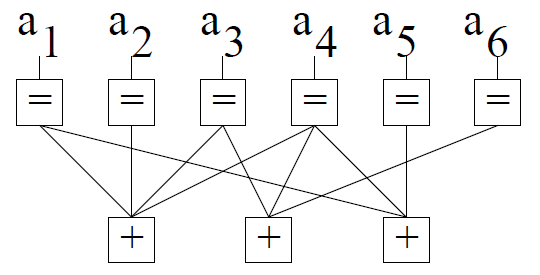
\includegraphics[width=150pt]{ldpc.png}
		\caption{Bipartitný graf reprezentujúci $(6,3)$-LDPC kód.}
	\end{figure}
	
	Majme kód reprezentovaný grafom vyššie.
	
	Kontrolnú maticu zostrojíme tak, že každý~$+$ vrchol bude reprezentovaný
	jedným riadkom, pričom tam bude $1$~pre každý $=$ vrchol, s~ktorým
	je tento $+$~vrchol spojený, $0$~pre ostatné.
	
	Pre kód zadaný daným grafom teda vyzerá kontrolná matica nasledovne:
	\[
		H =
		\begin{pmatrix}
			1 & 1 & 1 & 1 & 0 & 0 \\
			0 & 0 & 1 & 1 & 0 & 1 \\
			1 & 0 & 0 & 1 & 1 & 0 \\
		\end{pmatrix}
	\]
	
	Pre všetky slová tohto kódu potom platia nasledovné rovnosti:
	\[
		\begin{aligned} 
			a_1 + a_2 + a_3 + a_4 &= 0 \\
			a_3 + a_4 + a_6 &= 0 \\
			a_1 + a_4 + a_5 &= 0
		\end{aligned}
	\]
	
	Keď teda s použitím daného kódu obdržíme slovo $?01?11$, tak
	z~druhej rovnice vyplýva, že $a_4$~musí byť~$0$. Potom z~tretej
	rovnice vyplýva, že $a_1$~musí byť~$1$.
\end{example}


\subsection{Symetrická kryptografia}

V~symetrickej kryptografii obe strane zdieľajú jeden spoločný
tajný kľúč.

\begin{example}
	Príkladom je Caesarova šifra (posun každého písmena o konstantu).
	
	Nech Alica a Bob zdieľajú tajný kľúč $K=17$. Alica chce zakódovať 
	správu $m=\verb|INFORMATIKA JE SUPER|$. Zakódovaná správa po zakódovaní
	s~kľúčom $K=17$	bude $c=e_K(m)=\verb|ZEWFIDRKZBR AV JLGVI|$.
	
	Eva bez znalosti tajného kľúča nebude vedieť túto správu dekódovať
	(aj keď samozrejme Caesarova šifra môže mať najviac 26 rôznych kľúčov
	takže celkom jednoducho môže všetky vyskúšať). Bob so znalosťou 
	kľúča~$K$ jednoducho správu rozlúšti $m=d_K(c)$.
\end{example}

Ďalšími príkladmi sú Vigenèrova šifra (posun $n$-tic písmen, každé o různou konstantu).
Hillův kryptosystém (kódujeme $n$-tice násobením maticí-klíčem,
dekódujeme její inverzí). DES a AES.

Pre symetrickú kryptografiu by mali platiť nasledovné podmienky:
\begin{enumerate}
	\item So znalosťou kľúča~$K$ a funkcii~$e,d$ je ľahké spočítať
	$e_K(m)$ a $d_K(c)$.
	\item Zakódované $e_K(m)$ by nemalo byť o~moc dlhšie ako $m$.
	\item Malo by byť nemožné efektívne spočítať $d_K(c)$ bez znalosti
	funkcie~$d$ a kľúča~$K$.
	\item Malá zmena $m$ veľmi zmení $e_K(m)$.
	\item Množina kľúčov by mala byť veľká.
\end{enumerate}

Takisto by mali platiť podmienky \verb|CIAAN|:
\begin{itemize}
	\item \textsc{Confidentiality}: dáta môže dekódovať iba ten, 
	komu su určené
	\item \textsc{Integrity}: adresát si môže overiť, že dáta neboli 
	neautorizovane zmenené
	\item \textsc{Availability}: autorizovaní užívatelia musia mať
	prístup k~dátam a službám
	\item \textsc{Authenticity}: dáta pochádzajú od toho, od koho majú
	\item \textsc{Non-Repudiation}
\end{itemize}

Šifry sa dajú deliť na dva druhy - substitučné a transpozičné.

Substitučné nahradia časť textu časťou nejakého iného kryptotextu
podľa daných pravidiel. Môžu byť jednoduché (vždy na jedinom znaku),
monoalfabetické (zadané nejakou pevnou permutáciou),
polyalfabetické (môžu používať iné permutácie v~inej časti textu),
či polygrafické (menia naraz viac znakov).

Transpozičné šifry nemenia znaky, iba menia ich poradie v slove.

\begin{example}[Afinný kryptosystém]
	Afinný kryptosystém je špecifikovaný dvomi číslami $0 \leq a,b \leq 25$,
	$\gcd(a,26)=1$. Každý znak $x$ slova $m$ sa zakóduje ako $e_{a,b}(x)=(ax+b)\mod 26$.
	Dekóduje sa potom $d_{a,b}(y) = a^{-1}(y-b)\mod 26$.
\end{example}

\subsubsection{DES a AES}

DES rozdělí zprávu do 64-bitových bloků
a v~šestnácti krocích provádí nad každým blokem operace, které mají jako
argument také zvolený klíč. Argumentem operací může být i hodnota
předchozích bloků. Dešifrování spočívá v~pouhém obrácení pořadí operací.
8 bitů z~64 v~klíči je pro kontrolu parity, klíče jsou tedy prakticky
jen 56bitové.

DES byl nahrazen AES (ve verzi Rijndael [réndál]), který pracuje se
128bitovými bloky a až 256bitovými klíči. Dnes se používá například
k~šifrování disků nebo VPN.

Při šifrování AES používá matici $4 \times 4$ bytů a aplikuje na ni
postupně transformace (pro 256bitové klíče až 14 kol).
Jeden typ transformací jsou substituční tabulky,
další je posun bitů v řádcích,
ještě další je přehazování sloupců
a poslední je xor-ování sloupců s~klíčem.

\subsection{Asymetrická kryptografia}

V~kryptosystémech s~veřejným klíčem disponuje každý účastník dvěma
klíči: veřejným a soukromým. Uživatel může podepsat dokument svým
soukromým klíčem a každý potom může pomocí veřejného klíče ověřit
autenticitu dokumentu. Navíc každý může zašifrovat pomocí veřejného
klíče dokument, ten je pak dešifrovatelný pouze s~klíčem privátním.

\subsubsection{RSA}

Nejznámější kryptosystém s~veřejným klíčem je RSA, který je založený na
myšlence, že násobení čísel je snadné, zatímco na rozklad na prvočísla
dobrý algoritmus neznáme.

Pro ustanovení klíčů uživatel vygeneruje $s$-bitová prvočísla $p,q$
(typicky $s = 1024$), spočte $n = pq, \varphi(n) = (p-1)(q-1)$,
vybere velké $d$ tak, že $gcd(n, \varphi(n)) = 1$
a spočte $e = d^{-1} \mod \varphi(n)$. Veřejný klíč je tvořen dvojicí
$(n, e)$, soukromý klíč trojicí $p,q,d$.

Šifrujeme slowo $w$ výpočtem $c = w^e \bmod n$,
dešifrujeme $w = c^d \bmod n$.
Pro důkaz korektnosti potřebujeme Eulerovu větu $a^{\varphi(n)} = 1
\bmod \varphi(n)$ ($a,n$ jsou nesoudělná)
a Fermatovu větu $w^{p-1} = 1 \bmod p$ ($p$ je prvočíslo).
Pokud $p \nmid w, q \nmid w$, potom $gcd(n,w) = 1$, takže lze použít
Eulerovu větu a $c^d = w^{ed} = w^{j \varphi(n) + 1} = w \bmod n$.
Pokud $p \mid w$, ale $q \nmid w$,
pak snadno platí $w^{ed} = w \bmod p$
a navíc z~Fermatovy věty $w^{q-1} = 1 \bmod q$,
tedy
$w^{ed} = w^{ed - 1} w = w^{k(q-1)} w = (w^{q-1})^k w = 1^kw = w \bmod q$
a nakonec z Čínské zbytkové věty
$w^{ed} = w \bmod pq$.
Obě $p,q$ nemůžou dělit $w$, protože volíme čísla tak, aby $w < n$.

Prakticky zprávy kódujeme jako decimálně zapsané čísla,
rozdělené na bloky délky $i$ t.ž. $10^{i-1} \leq n < 10^i$.
Pro výpočet $w^e$ použijeme algoritmus binárního umocňování ({\em
exponentiation by squaring}).
Pro výpočet $d^{-1}$ použijeme rozšířený Euklidův
algoritmus.

% https://en.wikipedia.org/wiki/RSA_(cryptosystem)#Proofs_of_correctness

\subsubsection{Iné asymetrické kryptosystémy}
{\em Rabinov kryptosystém} je založený na tom, že modulo $n=pq$ je ľahké urobiť druhú
mocninu čísla, avšak odmocniť číslo je ťažké bez faktorizácie. Po odmocnení
vyjdú štyri odmocniny daného čísla, z~ktorých jedna je pôvodné slovo.

{\em Kryptosystém El~Gamal} je založený na diskrétnom logaritme. 
Verejným kľúčom je trojica $p,q,y$, kde $p$~je prvočíslo, $q$~je 
primitívny prvok $\mathbb{Z}^*_p$ a $y=q^x \mod p$. Súkromným kľúčom
je číslo $x < p$.

Slovo $w$ sa zakóduje pomocou náhodného čísla $r$ ako $a=q^r \mod p$,
$b=y^r w \mod p$. Kryptotextom je dvojica $(a,b)$.

Dekrypcia prebieha ako $w = \frac{b}{a^x}=ba^{-x}\mod p$.

\subsection{Kryptografie na eliptických křivkách}

Výhodou eliptických křivek je,
že pro zaručení stejné bezpečnosti jako použití běžných struktur (např.
$\mathbb{Z}_n$) stačí použít podstatně menších klíčů.

Eliptická křivka je graf bodů v~rovině splňujících
$y^2 = x^3 + ax + b \bmod n$, kde $a,b,n$ jsou celá čísla,
spolu s {\em bodem v nekonečnu}. Uvažujeme pouze křivky, kde neexistují
násobné kořeny (ekvivalentně $4a^3 + 27b^2 \neq 0$).

Pro každou křivku můžeme definovat sčítání tak, aby body spolu se
sčítáním tvořili komutativní grupu. Vzorce jsou poměrně komplikované,
příklad sčítání poskytne obrázek. Pomocí této grupy můžeme implementovat
například RSA.

\begin{figure}[H]
    \centering
    \includegraphics[width=200pt]{ec_add.png}
    \caption{Sčítání, \href{https://www.certicom.com/content/certicom/en/21-elliptic-curve-addition-a-geometric-approach.html}{zdroj}}
\end{figure}

Výhoda, kterou eliptické křivky poskytují, je v~podstatně složitějším
hádání klíčů, tedy stačí podstatně kratší klíče pro zajištění stejné
bezpečnosti jako u standradních postupů. Stejně jako pro čísla
pro křivky není známý rychlý
způsob výpočtu diskrétního logaritmu (tedy hledání $k$ takového, že $B =
kA$).

Nevýhodou je, že pro každé $x$ nemusí existovat $y$ a tedy některé
zprávy nejdou přímo zakódovat. Problém se řeší randomizovaným
algoritmem, který přidává několik bitů za takové zprávy.

\subsection{Schémata pro digitální podpisy}

Máme zprávu $m$, její hash $h(m)$. Chceme {\em podepsat} $h(m)$ (kvůli
efektivitě ne přímo $m$) funkcí $sig_{k_s}$ závislou na páru klíčů $(k_s,
k_p)$ a ověřit podpis funkcí $ver_{k_p}$.

Jedním schématem je \uv{obrácené RSA}. V~běžném RSA máme veřejné $n = pq$,
exponent $e$ a soukromý dešifrovací exponent $d$ a čísla $p,q$.
Šifrujeme zprávu $w$: $c = w^e$. Dešifrujeme $c$: $w = c^d$.
Podpis pomocí RSA se vytvoří $c = w^d$ a ověřuje se zda $w = c^e$.

Další schémata jsou například ElGamal či Rabinovo schéma.

\subsubsection{DSA}

Ako štandard pre podpisy bol vybraný DSA, ktorý vznikol modifikáciou
podpisov pomocou schématu El Gamal. Verejným kľúčom
je štvorica $(p,q,r,y)$, kde $p$ je prvočíslo, $q$ je prvočíslo, ktoré
delí $p-1$, $r=h^{(p-1)/q}\mod p$, kde $h$ je náhodný primitívny
prvok $\mathbb{Z}_p$, $r>1$ a $y=r^x\mod p$. Privátnym kľúčom
je hodnota $x$.

Podpis slova $w$ prebieha nasledovne: vyberie sa náhodné $k < q$.
Spočíta sa $a=(r^k\mod p) \mod q$, $b = k^{-1}(w+xa)\mod q$.
Podpisom je dvojica $(a,b)$.

Podpis sa overí tak, že sa spočíta $z=b^{-1}\mod q$, $u_1=wz\mod q$,
$u_2=az\mod q$. Potom sa overí, že $r^{u_1}y^{u_2}\mod q=a$.

\subsubsection{Fiat-Shamir}
V protokole Fiat-Shamir sa pre prvočísla $p,q$ spočíta $p \cdot q = n$,
ako verejný kľúč sa vyberú čísla $v_1, \ldots, v_k$ a ako súkromný kľúč
$s_1, \ldots, s_k$, $s_i=\sqrt{v_i^{-1}}\mod n$.

Podpis a overenie TODO

\subsection{Autentizační protokoly}

(Uvedeme jeden protokol. Profesor Gruska uvádí ještě dva, technicky
náročné protokoly jejichž memorování asi nemá větší význam.)

\begin{example}
Předpokládejme, že Alice a Bob sdíli tajný klíč $k$ a jednosměrnou
funkci $f_k$. Bob pošle Alici náhodné číslo $r$, Alice pošle Bobovi
$p = f_k(r)$ (tady by se Eva mohla pokusit o podvod posláním špatného
$p$), Bob ověří $p = f_k(r)$.
\end{example}

\subsection{Protokoly pro coin tossing}

{\em Házení mincí} je způsob digitálního hození mincí takový, že ani
jedna ze dvou stran nemůže výsledek určit, ale obě strany mohou hodnotu
ověřit.

Uvedeme dva protokoly. V~tom prvním Alice vybere jednosměrnou funkci $f$
a pošle Bobovi $f(0), f(1)$. Bob se pokusí uhádnout, které z $f(0), f(1)$
je výsledkem aplikace $f$ na $1$. Alice mu sdělí, zda je jeho odpověď
správná a pošle mu $f$, aby si mohl výsledek sám ověřit.

V tom druhém Alice vybere prvočísla $p,q$, pošle Bobovi $n = pq$.
Bob vybere $1 \leq x \leq n/2$, pošle alici $y = x^2 \bmod n$.
Alice vypočte všechny čtyři kořeny $x_1, n-x_1, x_2, n - x_2$ (spočte
nějakým algoritmem nebo zkusí možnosti modulo každé prvočíslo a pak použije CRT)
a tipem vybere jeden ze dvou,
které jsou menší než $n/2$.
Alica Bobovi nepošle svoj tip, ale dá mu vedieť, ktoré si vybrala (napr. 
vyberie nejaký bit, kde sa líšia, a pošle Bobovi poradie a hodnotu 
daného bitu).
Bob jí sdělí, zda trefila $x$ nebo ne a
pošle jí ho pro ověření, zatímco ona jemu pošle $p,q$ pro ověření.


\subsection{Protokoly pro bit commitment}

Účelem protokolů pro {\em závázní se k~bitu} je provedení volby, která
nelze jiným účastníkem předčasně odhalit, ale je možné ji po odhalení
ověřit.

Například Alice může bit napsat na papírek, umístit ho do truhly, tu
zamčít a dát Bobovi. Ve chvíli odhalení pak zkontroluje integritu truhly
a odemče ji svým klíčem.  Formálněji Alice zvolí jednosměrnou funkci
$f$, sudé (liché) $x$, pokud chce zakódovat $0$ ($1$) a pošle Bobovi
$(f, f(x))$.

U protokolů popisujeme {\em commitment phase} a {\em opening phase}.
Od protokolů očekáváme tři vlastnosti:
\begin{itemize}
    \item {\em hiding} -- Bob nemůže volbu Alice odhalit,
    \item {\em binding} -- Alice nemůže volbu skrytě změnit,
    \item {\em correctness} -- pokud vše probíhá dle protokolu, Bob se dozví správný bit.
\end{itemize}

Další protokol je například následující. Mějme prvočísla $p,q$,
číslo $n = pq$ a nakonec $m$ je kvandratický nezbytek\footnote{Tedy
neexistuje $x$ takové, že $x \bmod n = m$.} modulo $n$. Čísla $n, m$
zveřejníme.  Commitment je potom $f(b, x) = m^b x^2 \bmod n$ pro náhodně
zvolené $x \in \mathbb{Z}^*_n$. Protokol je hiding, protože výpočet
kvadratických zbytků je těžký. Protokol je binding, protože $m \in
QNR(n)$, a proto neexistují $x_1, x_2$ takové, že
$m x_1^2 = x_2^2 \bmod n$.


\subsection{Protokoly pro oblivious transfer}

Problém: Navrhnout protokol, který pošle zprávu od Alice Bobovi tak, že
Bob ji dostane s~pravděpodobností $1/2$. Bob ví, zda dostal zprávu nebo
chybnou zprávu, Alice to nezjistí.

Takový je například následující protokol:
\begin{enumerate}
    \item Alice zvolí dvě prvočísla $p,q$ a pošle Bobovi $n = pq$.
    \item Bob zvolí náhodně $x$ a pošle $y = x^2 \bmod n$.
    \item Alice spočte čtyři kořeny $y \bmod n$ a pošle jeden z~nich
        Bobovi.
    \item Bob ověří, jestli zaslaný kořen je kongruentní $x$. Pokud ano,
        nic se nedozvěděl. Pokud ne, má dva různé kořeny modulo $n$ a
        může tak faktorizovat~$n$. Alice se nic nedozvěděla.
\end{enumerate}

Můžeme také navrhnout protokol, ve kterém Alice pošle dvě zprávy a Bob
se dozví právě jednu z~nich a Alice se nedozví kterou.

\subsection{Steganografie a vodotisk}

Steganografie skrývá hlavní zprávu v~datech (například jako tajný přenos
dat), zatímco vodotisk je pouze
značkou umístěnou do hlavní zprávy (například pro kontrolu původu).

\begin{verbatim}
Příkladem,
a to ne moc dobrým,
steganografie v textu je
tento
asymetrický odstavec.
\end{verbatim}

Existují algoritmy pro vložení bitů do obrázků (jejich popis je
technický).

K digitálnímu vodotisku profesor Gruska říká pouze tolik, že jde o
vložení značky do dat tak, aby nešla odstranit nebo nejlépe ani
detekovat. Schmématem (bez bližšího vysvětlení) znázorňuje jak probíhá
vložení značky a její extrakce pro ověření. Rozlišuje míru znalostí pro
ověření: buď je potřeba originálu dat i verze s vodotiskem, nebo stačí
mít verzi s~vodotiskem.

% https://www.fi.muni.cz/usr/gruska/crypto17/cr1711.pdf

\subsection{Kryptografické stroje a jejich historie}

V~histórii kryptografie hovoríme o~štyroch obdobiach:
\begin{enumerate}
	\item Kryptografia bez strojov: lingvistické šifry (Caesar, Vigenère, Hill)
	\item Mechanická kryptografia: napr. Enigma
	\item Digitálna kryptografia: počítače, RSA, DSA, AES, ...
	\item Kvantová kryptografia
\end{enumerate}

Enigma byla vynalezena v~roce 1918. Má tři libovolně rotory, kde každá
pozice implementuje Caesarovu šifru. První rotor po napsání písmena
otočí o jedno dál a až obejde celou otáčku, tak posune o jedna další
rotor.  Navíc má Enigma desku pro transpozici písmen. Dohromady asi
$10^{16}$ možných konfigurací.

V~roce 1931 se dostaly do Francie dokumenty popisující zapojení rotorů.
Tento popis se dostal do rukou matematikovi Rejewskému,
který s~chytrým využitím teorie grup dokázal shrnout problém hledání
konfigurace Enigmy do několika rovnic.
Rejewski si navíc všiml, že Němci na začátku dne pro kontrolu dvakrát pošlou jednu
třípísmennou zprávu, což umožnilo redukovat počet možností pro kód
zvolený Němci pro daný den.

Rejewski měl k~dispozici model Enigmy pro komerční použití se zapojením
kláves v~běžném pořadí německých psacích strojů, $QWERTZU$\ldots Enigma
pro vojenské účely však měla klávesy v~pořadí $ABCDEF$\ldots -- tuto
možnost Britští kryptoanalytici ani nevyzkoušeli, jelikož ji považovali
za příliš zřejmou.

Rejewského tým navrhl mechanický počítač Bomba, který zkoušel již značně
omezený počet kombinací, což umožnilo dešifrovat zprávy z~Enigmy každý
den. Tuto technologii předali pět týdnu před začátkem války Francouzům a
Britům. Britský tým tuto technologii značně zdokonalil.

\subsection{Kvantová kryptografie}

Ve slidech profesora Grusky (které na přednášce neprobral)
a na Wikipedii.
% https://en.wikipedia.org/wiki/Quantum_key_distribution
% https://en.wikipedia.org/wiki/Quantum_teleportation

Pokúsim sa to tu nejako popísať, avšak za správnosť a úplnosť informácií
neručím.

Kvantová kryptografia je teoreticky absolútne bezpečná, fyzikálne
zákony zaručujú, že sa (v~istých prípadoch) nedá prelomiť. Kvantová
informácia sa ťažko ukladá a posiela, nie je možné ju skopírovať
a meraním sa zničí. Tento fakt prakticky znemožňuje man-in-the-middle
útoky, keďže pokiaľ by útočník informáciu získal, táto sa zničila
a on nie je schopný ju poslať ďalej; komunikujúce strany sa teda 
dozvedia o~útočníkovi. Kvôli tomuto v~kvantovej kryptografii
neexistuje spôsob ako vykonávať bit commitment a oblivious transfer.

V~kvantových počítačoch je informácia reprezentovaná qubitmi,
ktoré môžu mať ľubovoľnú z~nespočetného množstva hodnôt 
$\alpha|0\rangle + \beta|1\rangle$, kde $|\alpha|^2+|\beta|^2=1$ a 
$|\phi\rangle$ je stĺpcový vektor ekvivalentný $\phi$.

Qubit register môže mať naraz uložené všetky superpozície $2^n$.

\subsubsection{Generování náhodných tajných klasických klíčů}
Cieľom je využiť metód kvantovej kryptografie na vygenerovanie
náhodného tajného kľúča, ktorý bude mať Alica aj Bob, a Eva
nebude mať šancu ho zistiť.

Alica vygeneruje náhodný kľúč a posiela ho Bobovi nasledovne:
pre každý znak si vyberie náhodne bázu ($|0\rangle$, $|0'\rangle$,
resp. $|1\rangle$, $|1'\rangle$) a túto informáciu pošle Bobovi.

Bob prichádzajúce fotóny meria náhodne buď so štandardnou bázou~B
alebo s~duálnou bázou~D.

Pokiaľ meria s~bázou~B a Alica poslala buď $|0\rangle$ alebo $|1\rangle$,
Bob obdrží správnu hodnotu s~pravdepodobnosťou~1, inak je hodnota,
ktorú obdrží, dokonale náhodná.

Bob potom Alici pošle (klasickým kanálom) postupnosť báz, ktorú použil 
na meranie. Alica mu potom povie, ktoré bázy vybral správne,
a tieto hodnoty sú potom vybrané ako kľúč.

\begin{example}
	Alica posiela postupnosť \verb|10001100011| a posiela ju polarizovanú
	ako $|1\rangle|0'\rangle|0\rangle|0'\rangle|1\rangle|1'\rangle|0'\rangle|0\rangle|0\rangle|1\rangle|1'\rangle$.
	Bob použije na meranie postupnosť báz \verb|BDDDBBDBBDB| a obdrží
	postupnosť \verb|10001000010|.
	Po komunikácii klasickým kanálom vie, že obdržal postupnosť \verb|10R01R000RR|
	a kľúčom sa teda stáva postupnosť \verb|1001000|.
\end{example}

\subsubsection{Kvantová teleportace}
Princípom je, že Alica a Bob zdieľajú dve častice, ktoré
sú kvantovo prepojené.
\[
	|EPR_{pair}\rangle=\frac{1}{\sqrt{2}}(|00\rangle+|11\rangle)
\]
Potom stačí odmerať jednu z~častíc a meranie druhej častice je známe.
Toto sa dá využiť napríklad na zdieľanie symetrického kľúča.
